\subsection{Responzivní design}
Jednou z důležitých vlastností nové aplikace je nepochybně responzivní design, díky kterému je vzhled systému optimalizován pro klientské zařízení s různým rozlišením. S ohledem na skutečnost, že v dnešní době přistupuje na web nejvíce lidí z mobilních zařízení \cite{deviceusage}, je tato vlastnost o to zásadnější. Na obrázcích \ref{figure:homepage-responsive-layout} a \ref{figure:form-responsive-layout} je vidět způsob zobrazení hlavní stránky a stránky s formulářem pro přidání události na chytrém telefonu. Další ukázky z vytvořené aplikace jsou umístěny v příloze \ref{appendix}.

Vytvořený responzivní vzhled stojí z velké části na frameworku Bootstrap, který již byl představen v sekci \ref{bootstrap}. Příkladem části, jež Bootstrap kompletně neřeší, jsou tabulky. Pro ty byl s využitím jazyku JavaScript a CSS vytvořen mechanismus, který u zařízení s menším rozlišením postupně skrývá jednotlivé sloupce a naopak umožňuje zobrazení informací z těchto sloupců „rozbalením“ odpovídajícího řádku. Tato funkcionalita je demonstrována na obrázku \ref{figure:homepage-responsive-layout}.

\begin{figure}[h]
    \centering
    \begin{minipage}[b]{0.48\linewidth}
        \caption{Hlavní stránka}
        \label{figure:homepage-responsive-layout}
        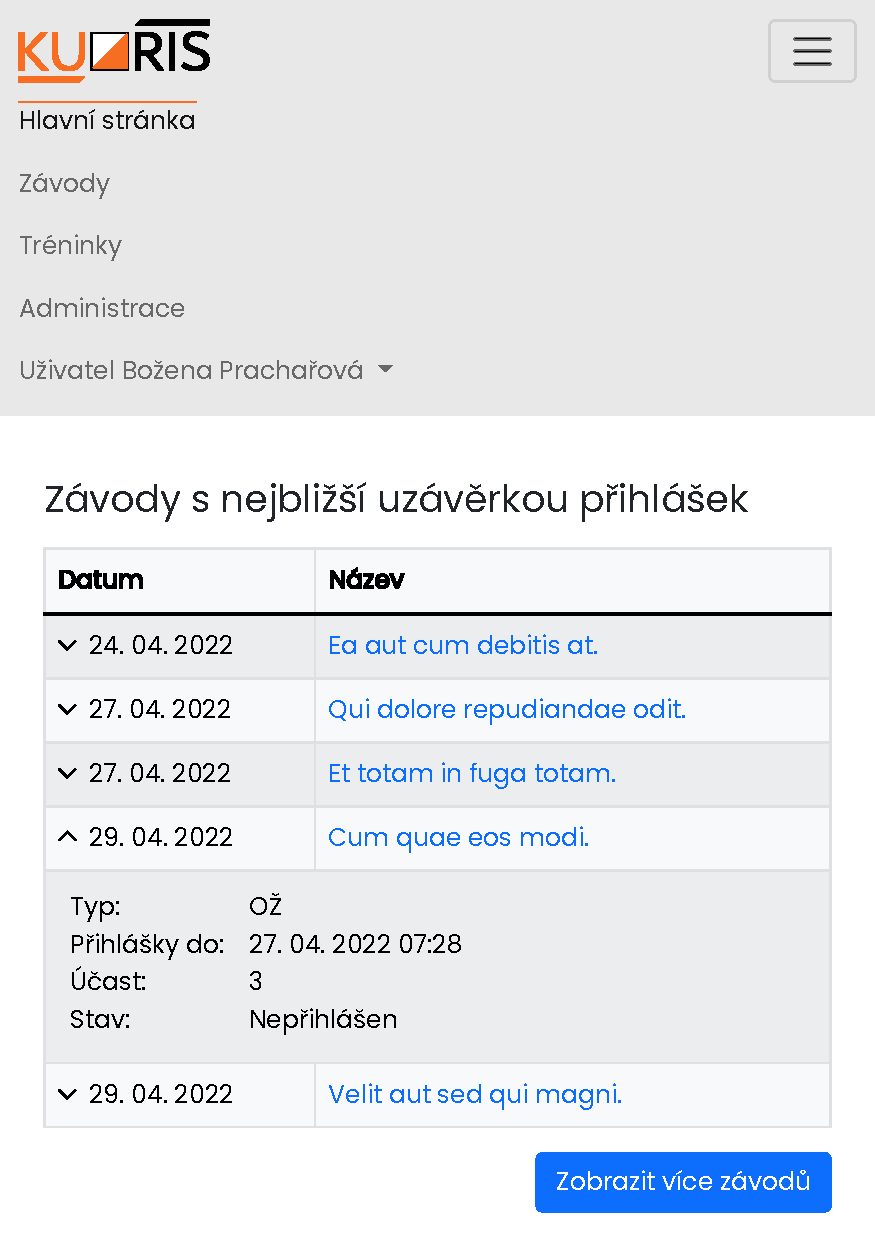
\includegraphics[width=0.99\linewidth, cfbox=kuorisgray 0.5pt 0pt]{images/homepage-responsive-layout.pdf}
    \end{minipage}
    \hfill
    \begin{minipage}[b]{0.48\linewidth}
        \caption{Formulář pro přidání události}
        \label{figure:form-responsive-layout}
        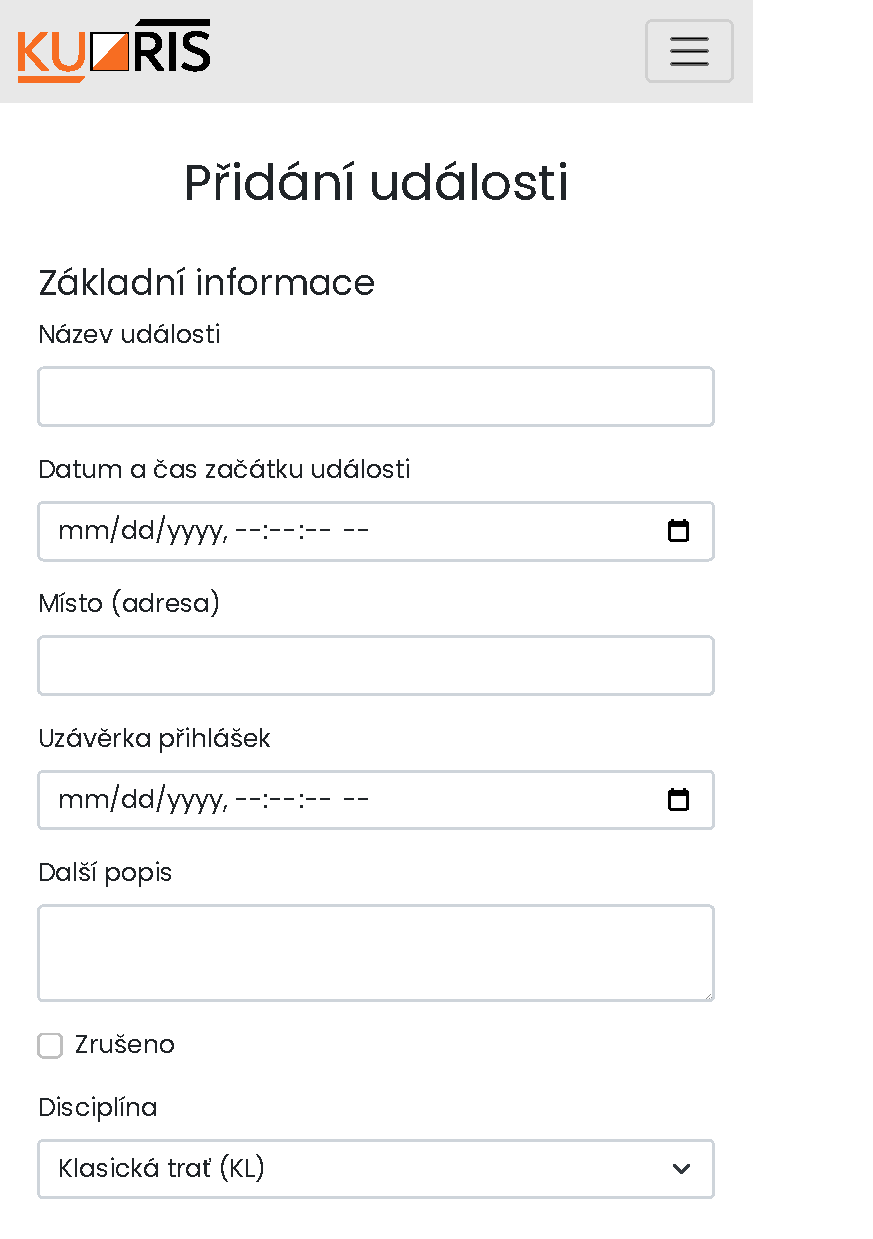
\includegraphics[width=0.99\linewidth, cfbox=kuorisgray 0.5pt 0pt]{images/form-responsive-layout.pdf}
    \end{minipage}
\end{figure}
